\chapter{Panel HMI}
\label{cha:panelHmi}

Głównym celem, do którego miało za zadanie prowadzić wybranie odpowiedniego algorytmu uczenia maszynowego do rozpoznawania głosowego było wykonanie panelu HMI. HMI (ang. Human-Machine Interface) jest to z definicji panel służący do połączenia człowieka z urządzeniem lub oprogramowaniem. Pomimo, że pojęcie to określa każdy ekran umożliwiający interakcję z maszyną, jest głównie używane w kontekście przemysłowym do komunikacji ze sterownikami PLC (ang. Programmable Logic Controllers). 
Panel HMI maszyny może być używany między innymi do:
\begin{itemize}
    \item sterowania,
    \item monitorowania wejść i wyjść,
    \item wizualizacji danych,
    \item śledzenia procesów.
\end{itemize}
Panele takie często są budowane do wytrzymywania w ekstremalnych warunkach w zakładach przemysłowych i fabrykach i przystosowywane do działania na odległość. Ich powstanie jest powiązane głównie z potrzebą optymalizacji - dzięki urządzeniom monitorującym procesy zdalnie, pracownicy zakładów zamiast marnować czas na sprawdzanie każdej maszyny, mogą to zrobić w jednym, dedykowanym do tego miejscu. 

%---------------------------------------------------------------------------

\section{Środowisko pracy}
\label{sec:srodPrac}

Stanowiskiem pracy jest urządzenie z systemem operacyjnym Ubuntu 20.04. W celach użycia narzędzia \textit{Gazebo} \cite{gazebo} służącego do symulowania systemów w czasie rzeczywistym, zainstalowano środowisko \textit{Robot Operating System} (skr.: ROS) \cite{ros}. 

ROS \cite{ros} jest to otwarte oprogramowanie posiadające zestaw bibliotek i narzędzi umożliwiający budowanie aplikacji dla robotów, kompatybilne z językiem programowania \textit{Python}. Dystrybucja zainstalowana na urządzeniu to \textit{ROS Noetic Ninjemys} \cite{noetic}, odmiana dedykowana dla używanego systemu operacyjnego z długoterminowym wsparciem ze strony producenta. 

Do zobrazowania działania algorytmu w symulacji został użyty model TurtleBot3 \cite{turtlebot}. Jest to robot, którego nazwa, wygląd, a nawet sposób poruszania bazuje na Turtle, popularnym robocie będącym integralną częścią języka programowania Logo \cite{logo}. Wybrany model robota to \textit{waffle} \ref{fig:gazebo}.

\begin{center}
    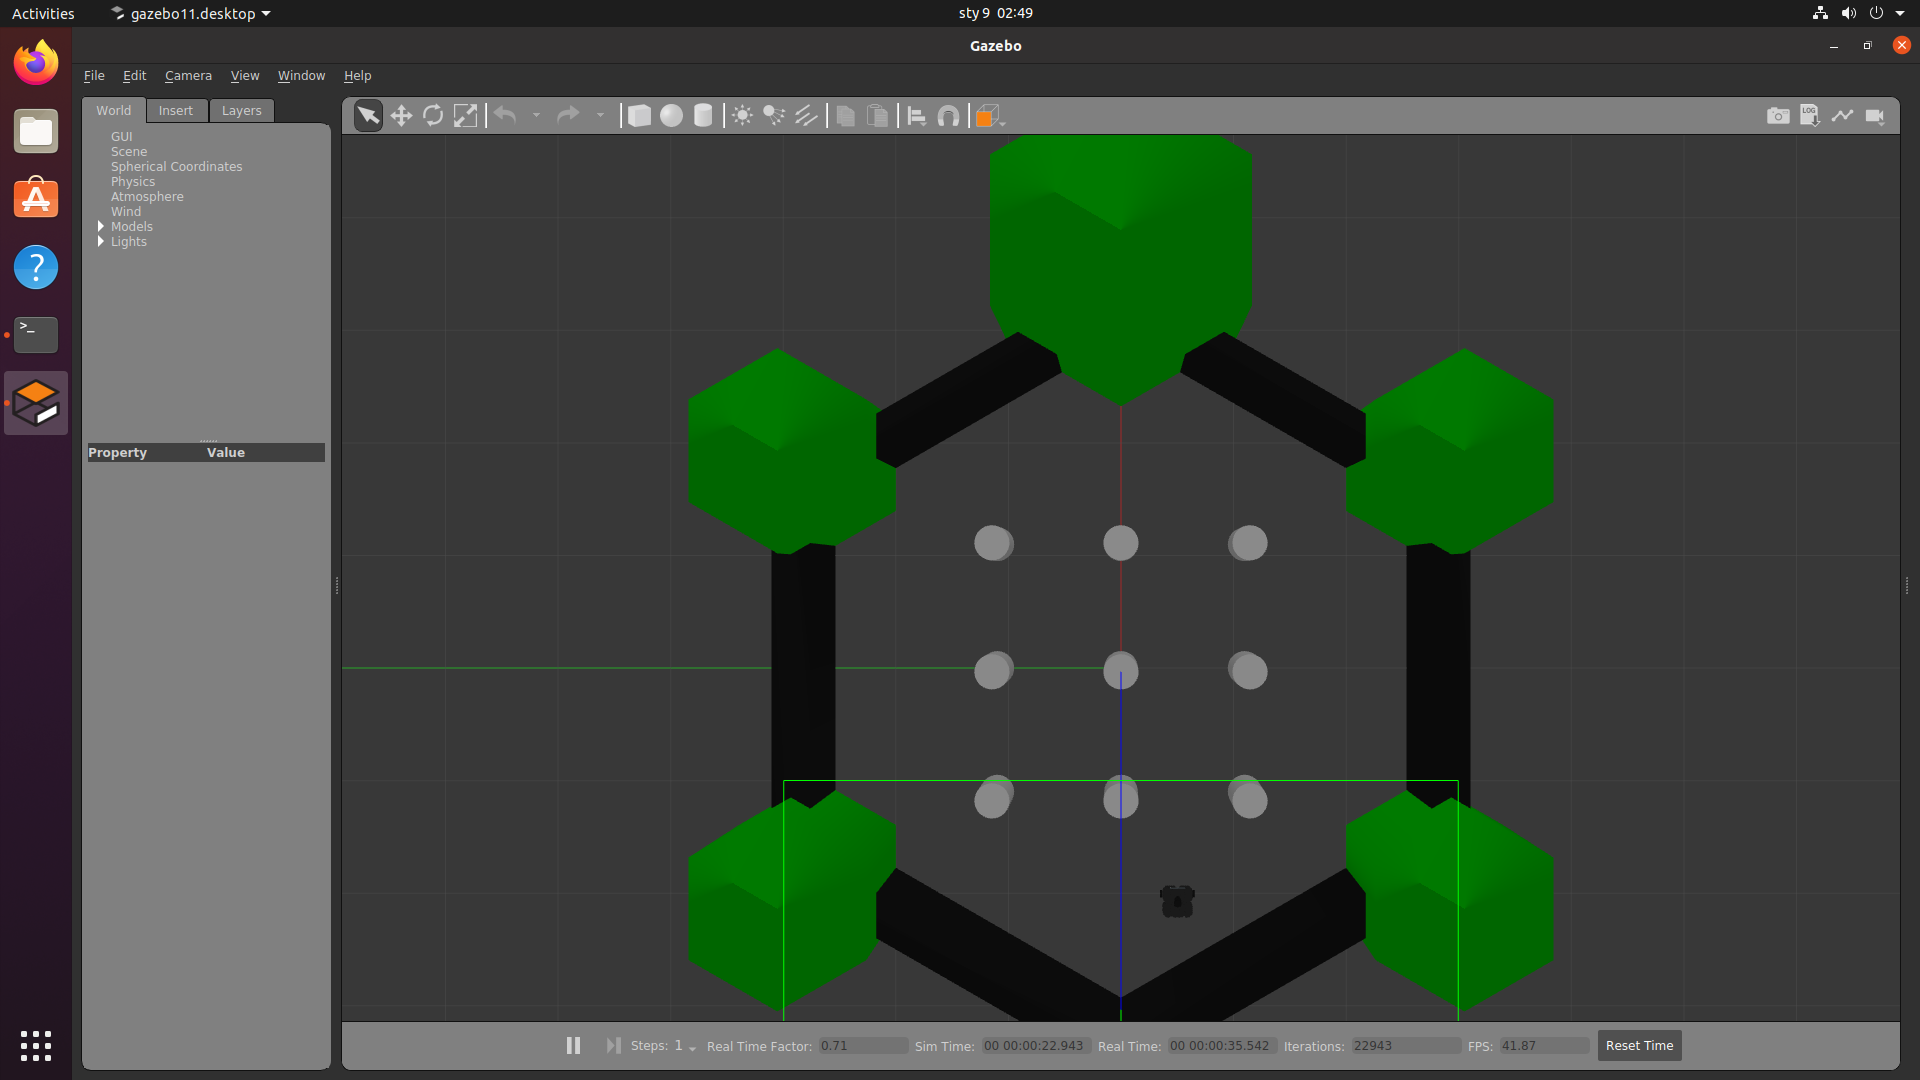
\includegraphics[width=0.8\linewidth]{files/gazebo.png}
    \captionof{figure}{Widok aplikacji Gazebo wraz z uruchomioną symulacją robota.}
    \label{fig:gazebo}
\end{center}

Monitorowanie zaimplementowanego sterowania robotem umożliwia narzędzie \textit{rqt} \cite{rqt}. Jest to oprogramowanie zapewniające szeroki zakres wtyczek do wizualizacji wszelkiego rodzaju danych. Na Rys. \ref{fig:rqt} widoczny jest przykładowy wykres prędkości liniowej kół robota w osi x w czasie. 

\begin{center}
    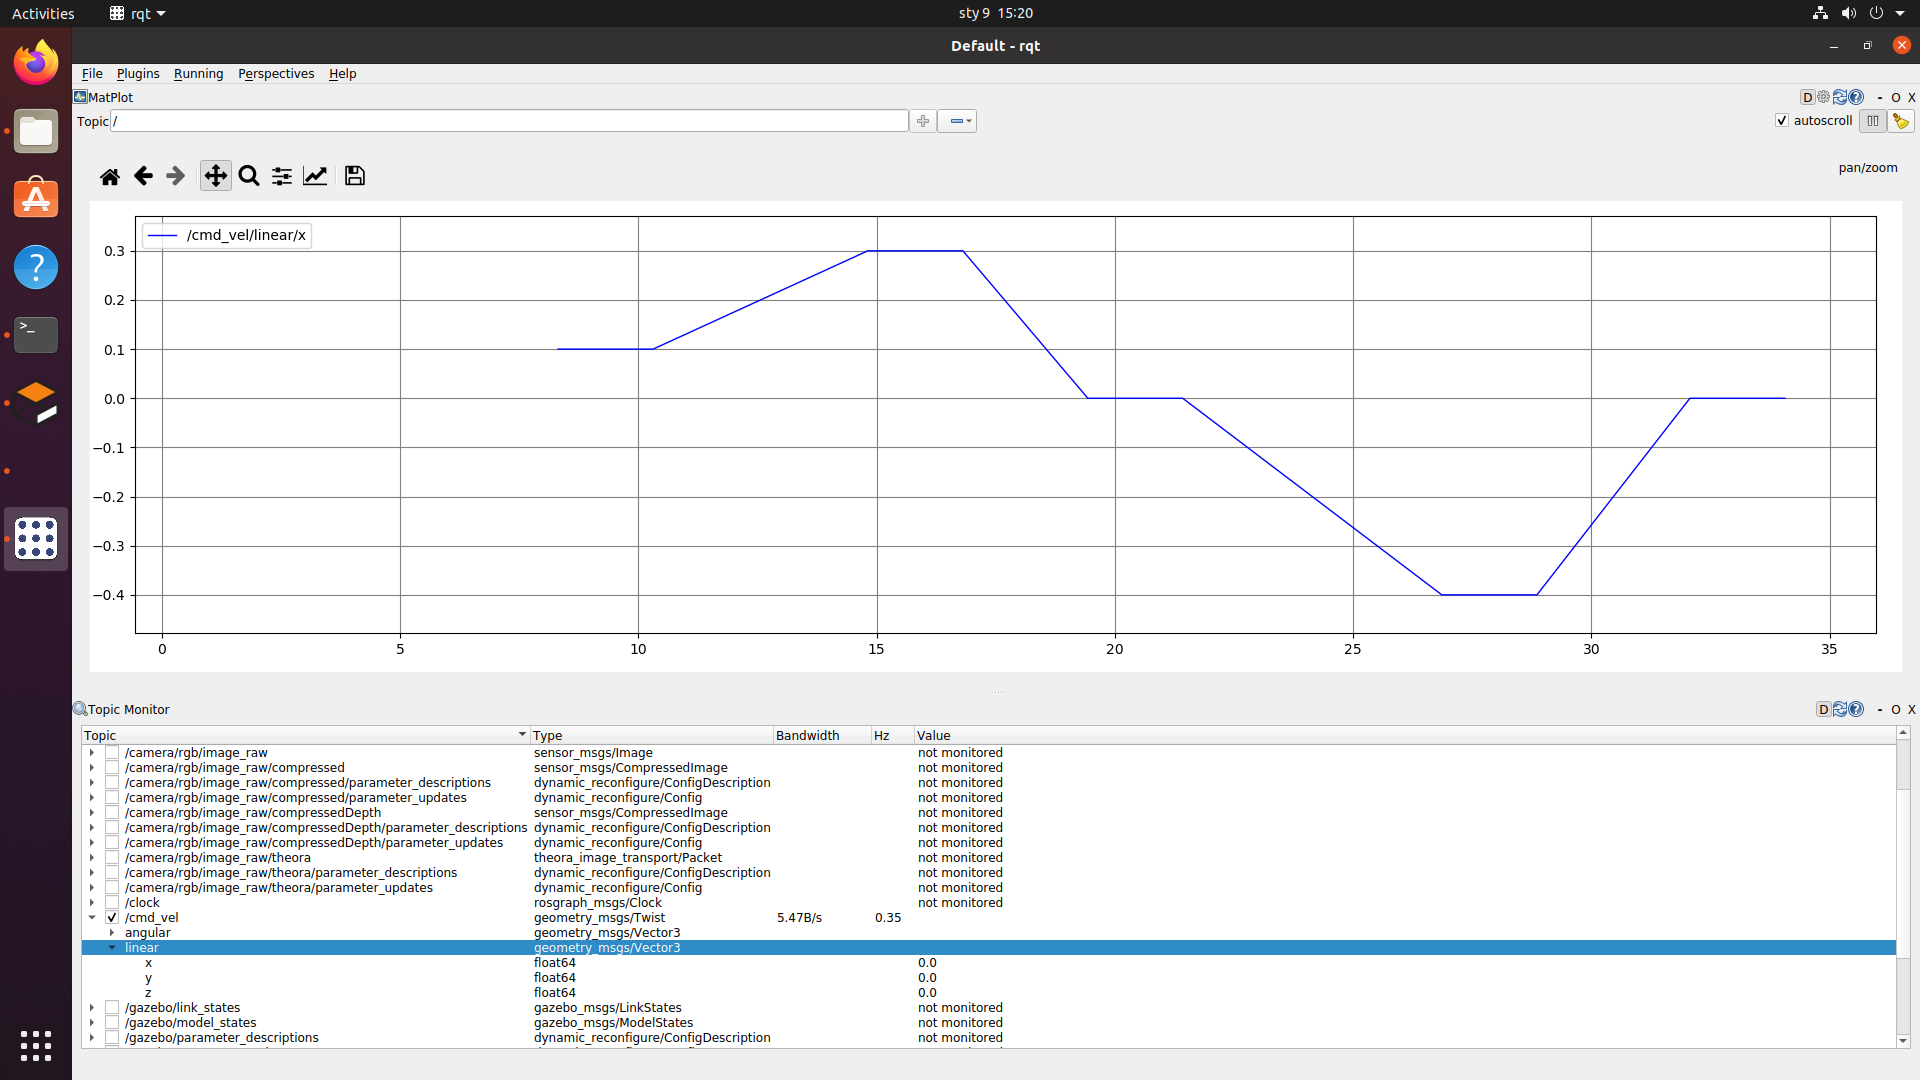
\includegraphics[width=0.8\linewidth]{files/rqt_view.png}
    \captionof{figure}{Widok aplikacji rqt.}
    \label{fig:rqt}
\end{center}

Wymienione powyżej narzędzia służą głównie usprawnieniu pracy w środowisku i weryfikacji założeń projektowych. Sam przebieg działania programu, widoczny na Rys. \ref{fig:diagram} przedstawia się następująco: po starcie programu pojawia się panel do sterowania, który odbiera dane wejściowe audio. Dane te są przekazywane do algorytmu używanego do rozpoznawania mowy, który konwertuje je na komendy. Panel do sterowania przekazuje te komendy robotowi umieszczonemu w symulacji, a ich wykonanie może być odczytane z wykresu.

\begin{center}
    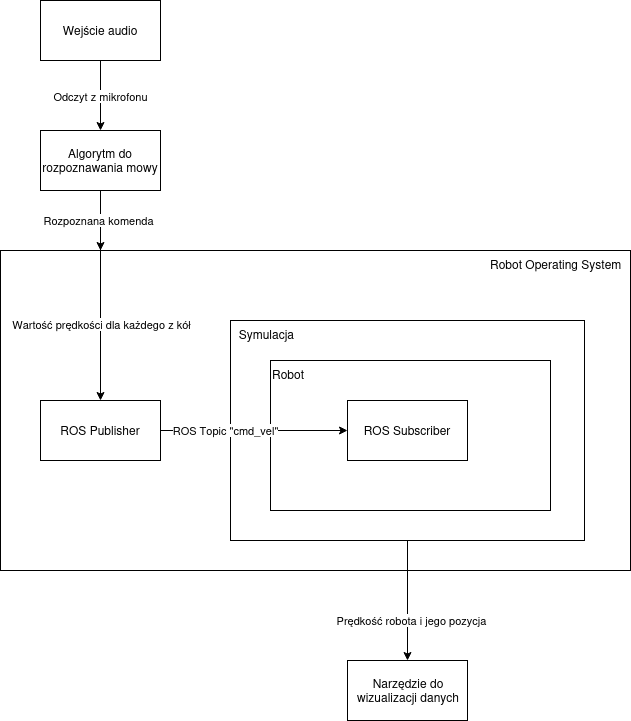
\includegraphics[width=0.95\linewidth]{files/diagram.png}
    \captionof{figure}{Diagram przedstawiający proces działania programu.}
    \label{fig:diagram}
\end{center}

Samo przekazanie przez panel komend robotowi odbywa się za pomocą narzędzia \textit{ROS Topic} (z ang. tematy). Tematami w środowisku ROS można określić instancje odpowiedzialne za przekazywanie wiadomości (ang. \textit{messages}) pomiędzy węzłami (ang.\textit{nodes}). Aby nadać jakąś wiadomość na dany temat używany jest \textit{ROS Publisher} (z ang. nadawca). Wiadomość taką może odebrać \textit{ROS Subscriber} (z ang. odbiorca). W widocznym na Rys. \ref{fig:diagram} przebiegu programu, aby umożliwić poruszanie się robota, na temat \textit{cmd-vel}, odpowiedzialny za prędkość kół robota, nadawana jest wiadomość zawierająca pożądaną wartość prędkości kół. Robot, jako subskrybent tego tematu odbiera wiadomość w tym temacie i zaczyna poruszanie się z tą prędkością. 

%---------------------------------------------------------------------------

\section{Aplikacja}
\label{sec:App}

W projekcie w celu wykonania panelu służącego do sterowania głosowego urządzeniem użyto biblioteki dla Pythona \textit{CustomTkinter} \cite{ctk}. Umożliwia ona prostą w obsłudze budowę aplikacji i dostosowanie ich pod potrzeby wizualne użytkownika. 

Podstawowym elementem programu jest widoczny na Rys. \ref{fig:panel_1} panel. Przyciski \textit{start} oraz \textit{stop} służą do zmiany stanu robota na ruch lub oczekiwanie. Przy przycisku \textit{start} znajduje się opcjonalne pole służące do wprowadzenia prędkości poruszania się robota. Przycisk \textit{voice recognition} otwiera okno służące do sterowania głosowego \ref{fig:panel_2}.
\begin{center}
    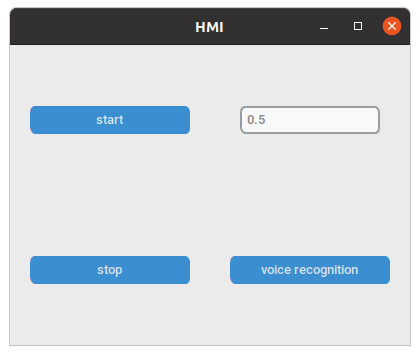
\includegraphics[width=0.95\linewidth]{files/panel_1.png}
    \captionof{figure}{Główne okno panelu HMI.}
    \label{fig:panel_1}
\end{center}

Widoczny na Rys. \ref{fig:panel_2} panel posiada przycik \textit{start/stop speaking} uruchamiający lub zatrzymujący sterowanie głosowe. Ponad to, na polu obok wyświetlane są komendy programu w czasie rzeczywistym. 

\begin{center}
    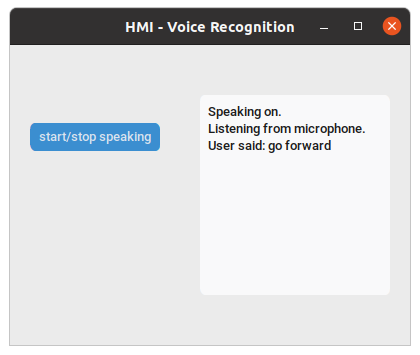
\includegraphics[width=0.95\linewidth]{files/panel_2.png}
    \captionof{figure}{Okno panelu HMI służące do sterowania głosowego.}
    \label{fig:panel_2}
\end{center}

Sterowanie może przebiegać za pomocą ...
dwa panele
rtq
poruszanie sie liniowe i angular